\documentclass[a4paper,10pt]{article}

%\usepackage{xltxtra}
\usepackage{fontspec, unicode-math}
\usepackage{amsmath}
\usepackage{hyperref}

\usepackage[]{biblatex}
\addbibresource{Notes-ref.bib}

\usepackage[siunitx, americanvoltage]{circuitikz}
\usepackage{tikz}
\usetikzlibrary{patterns,decorations.pathmorphing,shapes,arrows,positioning,decorations.pathreplacing,calc,backgrounds,external,spy}

\setromanfont[Mapping=tex-text]{Linux Libertine O}
% \setsansfont[Mapping=tex-text]{DejaVu Sans}
% \setmonofont[Mapping=tex-text]{DejaVu Sans Mono}

\title{Notes on Vacuum Electronics Molecular Dynamics Simulations}
\author{Kristinn Torfason}
\date{\today}

\newcommand{\ud}{\mathrm{d}}

\begin{document}
\maketitle\thispagestyle{empty}
\newpage

\section{Verlet Integration}
\begin{equation}
\mathbf{x}_{n+1} = 2\mathbf{x}_{n} - \mathbf{x}_{n-1} + \frac{\mathbf{F}_{n}(\mathbf{x}_{n})}{m} {\Delta t}^{2}
\end{equation}
Force on a particle at \(\mathbf{r}\) due to all other particles at positions \(\mathbf{r}_i\)
\begin{equation}
  \mathbf{F}(\mathbf{r}) = \frac{q^2}{4\pi\varepsilon_0} \sum_{i=1}^{N} \frac{\mathbf{r} - \mathbf{r}_i}{|\mathbf{r} - \mathbf{r}_i|^3}
\end{equation}
Force on a particle due to an electric field
\begin{equation}
  F(\mathbf{r}) = qE(\mathbf{r})
\end{equation}
in case of a constant field in the \(z\)-direction \(\mathbf{E} = \left[ 0, 0, E_z \right]\)
\begin{equation}
 F_z = qE_z = q \frac{V}{d},
\end{equation}
where \(V\) is the voltage and \(d\) the gap distance.
Initial fictitious previous position
\begin{equation}
 x_{n-1} = x_n - v_0{\Delta t} - \frac{F(x_n)}{2 m} {\Delta t}^2\,
\end{equation}
where \(v_0\) is the initial velocity.

\subsection{Velocity Verlet}
  The Velocity Verlet method is done in three steps, fyrst update the position,
  \begin{equation}
    x_{n+1} = x_n + v_n\Delta t + \frac{1}{2}a_n{\Delta t}^2\, ,
  \end{equation}
  then calculate the acceleration \(a_{n+1}\) using \(x_{n+1}\) and finaly
  update the velocity,
  \begin{equation}
    v_{n+1} = v_n \frac{a_n + a_{n+1}}{2}{\Delta t}^2\, .
  \end{equation}
  Note this method assumes that \(a_{n+1}\) dose not depend on \(v_{n+1}\).
  This could be a problem when using a magnetic field which depends on the
  velocity. First approximation would be to use \(v_n\) if the field is week,
  see also~\cite{SPREITER1999102}.

\subsubsection{Nondimensionalization}
  Set \(x_n = L \bar{x}_n\), where \(L\) is a characteristics length scale and
  \(\bar{x}_n\) is a dimensionless length. Similarly set \(v_n = T \bar{v}_n\)
  where \(T\) is a characteristics time scale for the system.
  Then \(\Delta t = T\Delta \bar{t}\) and \(a_n = \frac{L}{T^2}\bar{a}_n\).
  The equations then become,
  \begin{equation}
    \bar{x}_{n+1} = \bar{x}_n + \bar{v}_n\Delta \bar{t} + \frac{1}{2}\bar{a}_n{\Delta \bar{t}}^2\, ,
  \end{equation}
  and,
  \begin{equation}
    \bar{v}_{n+1} = \bar{v}_n \frac{\bar{a}_n + \bar{a}_{n+1}}{2}{\Delta \bar{t}}^2\, .
  \end{equation}
  In program \(L = 1.0*10^{-9}\,\mathrm{m}\) and \(T = 1.0*10^{-12}\,\mathrm{s}\),
  i.e. lengths are scaled in nano-meters and time in pico-seconds.

\section{Field Emission}
\subsection{Fowler-Nordheim equation}
\begin{equation}
  J = \frac{a}{\phi t^2(l)}F^2 exp(-\nu(l)b\phi^{3/2}/F)
\end{equation}
where \(a \approx 1.541434\times 10^{-6}\,\mathrm{AeVV^{-2}}\) and \(b \approx 6.830890\,\mathrm{eV^{-3/2} V nm^{-1}}\) are
the first and second Fowler-Nordheim constants (see equation~\eqref{eq:a_fn} and~\eqref{eq:b_fn}).

The equation for \(\nu(l)\) is~\cite{Forbes08112007}
\begin{equation}
 \nu(l) = 1 - l + \frac{1}{6}l \ln(l)
\end{equation}
and for \(t(l)\)
\begin{equation}
  t(l) = 1 + l\left( \frac{1}{9} - \frac{1}{18}\ln(l) \right)
\end{equation}
where
\begin{equation}
 l = \frac{F}{F_\phi} = \frac{e^3}{4\pi\epsilon_0} \frac{F}{\phi^2}
\end{equation}
If \(\phi\) is in eV and \(F\) in V/m then
\begin{equation}
  l = \frac{e}{4\pi\epsilon_0} \frac{F}{\phi^2}
\end{equation}

The first Fowler-Nordheim constant is in SI units
\begin{equation}\label{eq:a_fn}
 a_{FN} = \frac{e^3}{8\pi h}
\end{equation}
and has units \(\mathrm{A}\mathrm{J}\mathrm{V}^{-2}\). If we convert to \(\mathrm{A}\mathrm{eV}\mathrm{V}^{-2}\) then
we must multiply with \(1/e\) to obtain
\begin{equation}\label{eq:b_fn}
 a_{FN} = \frac{e^2}{8\pi h} = \frac{e^2}{16\pi^2 \hbar}
\end{equation}
The second Fowler-Nordheim constant is in SI units
\begin{equation}
  b_{FN} = \frac{8\pi}{3eh}\sqrt{2m_e}
\end{equation}
and has the units \(\mathrm{J}^{-3/2}\mathrm{V}\mathrm{m}^{-1}\). If we convert it to \(\mathrm{eV}^{-3/2}\mathrm{V}\mathrm{m}^{-1}\) then
we must multiply it with a factor of \((1/e)^{-3/2}\) and obtain
\begin{equation}
 b_{FN} = \frac{8\pi\sqrt{2m_e e}}{3h} = \frac{4}{3\hbar}\sqrt{2em_e}
\end{equation}

\subsection{Surface Field Calculations}
If we assume a box with height \(d\) in \(z\), length \(L\) in \(x\) and \(y\), with a charge density \(\sigma(z)\).
Then the surface field at the middle of the bottom in the \(z\) direction is given by
\begin{equation}
  E = E_0 + 2\int\limits_0^d\!\! \int\limits_{-\frac{L}{2}}^{\frac{L}{2}}\!\! \int\limits_{-\frac{L}{2}}^{\frac{L}{2}}\!\!
    \frac{1}{4\pi\epsilon_0} \frac{z \sigma(z)}{(x^2 + y^2 + z^2)^{3/2}}\, \ud x\, \ud y\, \ud z\, .
\end{equation}
The factor of two before the integral is to account for image charge effects.
If all lengths are scaled with the gap spacing \(d\), \(\hat{x} = x/d\), \(\hat{y} = y/d\) and \(\hat{z} = z/d\).
Charge density scaled with \(\sigma_0 = 4\pi V_0 \epsilon_0/d^2\), which leads to that current density is scaled
by the Child Langmuire limit \(\hat{J} = J/J_{CL}\), or \(\hat{\sigma}(\hat{z}) = \hat{J}/9\pi\sqrt{\hat{z}}\).
The field is scaled by the vacuum field \(E_0 = -V_0/d\), we then obtain
\begin{equation}
  E = 1 - \frac{2J}{9\pi}\int\limits_0^1\!\! \int\limits_{-\frac{L}{2d}}^{\frac{L}{2d}}\!\! \int\limits_{-\frac{L}{2d}}^{\frac{L}{2d}}\!\!
    \frac{\sqrt{\hat{z}}}{(\hat{x}^2 + \hat{y}^2 + \hat{z}^2)^{3/2}}\, \ud \hat{x}\, \ud \hat{y}\, \ud \hat{z}\, .
\end{equation}
Calculated iteratively


\cleardoublepage
\subsection{Prolate spheroidal coordinates}
  The prolate spheroidal coordinates are defined as
  \begin{equation}\begin{split}
    x &= a \sinh{\mu}\sin{\nu}\cos{\phi}\\
    y &= a \sinh{\mu}\sin{\nu}\sin{\phi}\\
    z &= a \cosh{\mu}\cos{\nu}
  \end{split}\end{equation}
  Set \(\xi = \cosh{\mu}\) and \(\eta = \cos{\nu}\) then
  \begin{equation}\begin{split}
    \sinh^2{\mu} &= \cosh^2{\mu} - 1 = \xi^2 - 1\\
    \sin^2{\nu}  &= 1 - \cos^2{\nu} = 1 - \eta^2
  \end{split}\end{equation}
  which gives
  \begin{equation}\begin{split}
    x &= a \sqrt{\xi^2-1}\sqrt{1-\eta^2} \cos{\phi}\\
    y &= a \sqrt{\xi^2-1}\sqrt{1-\eta^2} \sin{\phi}\\
    z &= a \xi \eta
  \end{split}\end{equation}
  The reverse are
  \begin{equation}\begin{split}
    \xi &= \frac{1}{2a} \left( \sqrt{x^2 + y^2 + (z+a)^2} + \sqrt{x^2 + y^2 + (z-a)^2} \right)\\
    \eta &= \frac{1}{2a} \left( \sqrt{x^2 + y^2 + (z+a)^2} - \sqrt{x^2 + y^2 + (z-a)^2} \right)\\
    \phi &= \arctan{\frac{y}{x}}
  \end{split}\end{equation}
  To find \(\xi\) or \(z\) if given \(x\) and \(y\)
  \begin{equation}
    \xi = \frac{1}{a\sqrt{1-\eta^2}}\sqrt{x^2 + y^2 + a^2(1-\eta^2)}
  \end{equation}
  \begin{equation}
    z = \frac{\eta}{\sqrt{1-\eta^2}}\sqrt{x^2 + y^2 + a^2(1-\eta^2)}
  \end{equation}
  Derivatives of the coordinates
  \begin{equation}\begin{split}
    \frac{\partial x}{\partial \xi} = a\xi \frac{\sqrt{1-\eta^2}}{\sqrt{\xi^2-1}} \cos{\phi}\, ,\quad
      \frac{\partial y}{\partial \xi} &= a\xi \frac{\sqrt{1-\eta^2}}{\sqrt{\xi^2-1}} \sin{\phi}\, ,\quad
      \frac{\partial z}{\partial \xi} = a\eta\, ,\\
    \frac{\partial x}{\partial \eta} = -a\eta \frac{\sqrt{\xi^2-1}}{\sqrt{1-\eta^2}} \cos{\phi}\, ,\quad
      \frac{\partial y}{\partial \eta} &= -a\eta \frac{\sqrt{\xi^2-1}}{\sqrt{1-\eta^2}} \sin{\phi}\, ,\quad
      \frac{\partial z}{\partial \eta} = a\xi\, ,\\
    \frac{\partial x}{\partial \phi} = -a\sqrt{\xi^2-1}\sqrt{1-\eta^2} \sin{\phi}\, ,\quad
      \frac{\partial y}{\partial \phi} &= a\sqrt{\xi^2-1}\sqrt{1-\eta^2} \cos{\phi}\, ,\quad
      \frac{\partial z}{\partial \phi} = 0\, .
  \end{split}\end{equation}

  The gradient is
  \begin{equation}\begin{split}
   \nabla V(\xi, \eta, \phi) &= \hat{x} \frac{\partial V}{\partial x} + \hat{y} \frac{\partial V}{\partial y} + \hat{z} \frac{\partial V}{\partial z} \\
                             &= \hat{x} \left( \frac{\partial V}{\partial \xi} \frac{\partial \xi}{x}
                                + \frac{\partial V}{\partial \eta} \frac{\partial \eta}{x}
                                + \frac{\partial V}{\partial \phi} \frac{\partial \phi}{x} \right) \\
                             &+ \hat{y} \left( \frac{\partial V}{\partial \xi} \frac{\partial \xi}{y}
                                + \frac{\partial V}{\partial \eta} \frac{\partial \eta}{y}
                                + \frac{\partial V}{\partial \phi} \frac{\partial \phi}{y} \right) \\
                             &+ \hat{z} \left( \frac{\partial V}{\partial \xi} \frac{\partial \xi}{z}
                                + \frac{\partial V}{\partial \eta} \frac{\partial \eta}{z}
                                + \frac{\partial V}{\partial \phi} \frac{\partial \phi}{z} \right)
  \end{split}\end{equation}
  The position vector is
  \begin{equation}
   \vec{r} = \begin{pmatrix}
               a \sqrt{(\xi^2-1)(1-\eta^2)}\cos{\phi}\\
               a \sqrt{(\xi^2-1)(1-\eta^2)}\sin{\phi}\\
               a\xi\eta
             \end{pmatrix}\, ,
  \end{equation}
  and the unit vector are then
  \begin{equation}
    \hat{\xi} = \frac{\frac{\ud \vec{r}}{\ud \xi}}{\left|\frac{\ud \vec{r}}{\ud \xi}\right|}\,, \quad
    \hat{\eta} = \frac{\frac{\ud \vec{r}}{\ud \eta}}{\left|\frac{\ud \vec{r}}{\ud \eta}\right|}\,, \quad
    \hat{\phi} = \frac{\frac{\ud \vec{r}}{\ud \phi}}{\left|\frac{\ud \vec{r}}{\ud \phi}\right|}\, .
  \end{equation}
  For \(\hat{\eta}\) we have
  \begin{equation}
   \hat{\eta} = \sqrt{\frac{1-\eta^2}{\xi^2-\eta^2}}
     \begin{pmatrix}
       -\eta \sqrt{\frac{\xi^2-1}{1-\eta^2}} \cos{\phi}\\
       -\eta \sqrt{\frac{\xi^2-1}{1-\eta^2}} \sin{\phi}\\
       \xi
     \end{pmatrix}
  \end{equation}
  Scale factors are
  \begin{equation}
    h_{\xi} = a \sqrt{ \frac{\xi^2-\eta^2}{\xi^2-1} }\,, \quad
  %\end{equation}
  %\begin{equation}
    h_{\eta} = a \sqrt{ \frac{\xi^2-\eta^2}{1-\eta^2} }\,, \quad
  %\end{equation}
  %\begin{equation}
    h_{\phi} = a \sqrt{ (\xi^2-1)(1-\eta^2) }
  \end{equation}
%
  Given \(x\), \(y\) and \(\eta_1\)
  \begin{equation}
   \xi = \frac{1}{a} \frac{1}{\sqrt{1-\eta_1^2}} \sqrt{x^2 + y^2 + a^2(1-\eta_1^2)}
  \end{equation}
%
%
\subsection{Electric field for hyperbolid tip}
  The vector potential is~\cite{pan:2151}
  \begin{equation}
    V(\eta) = V_0 \frac{\ln{\left[ \frac{1 + \eta_1}{1-\eta_1}\frac{1-\eta}{1+\eta} \right]}}{\ln{\left[ \frac{1+\eta_1}{1-\eta_1}\frac{1-\eta_2}{1+\eta_2} \right]}}\, .
  \end{equation}
  The boundary conditions have been swaped from Ref.~\parencite{pan:2151}. The tip is now held at \(V = 0\) and the anode at \(V = V_0\).
  The derivative of the potential is
  \begin{equation}
    \frac{\ud V(\eta)}{\ud \eta} = -\frac{2V_0}{1-\eta^2} \ln^{-1} \left[ \frac{1+\eta_1}{1-\eta_1} \frac{1-\eta_2}{1+\eta_2} \right]
  \end{equation}
  The gradient in Prolate-Spherodial coordinates is
  \begin{equation}
    \nabla V(\eta) = \frac{1}{a} \sqrt{\frac{1-\eta^2}{\xi^2-\eta^2}} \frac{\ud V(\eta)}{\ud \eta} \hat{\eta}\, ,
  \end{equation}
  and the electric field is
  \begin{equation}
   \vec{E} = - \nabla V(\eta) = \frac{2V_0}{a} \frac{1}{\xi^2-\eta^2} \frac{1}{\ln \left[ \frac{1+\eta_1}{1-\eta_1} \frac{1-\eta_2}{1+\eta_2} \right]}
                                \begin{pmatrix}
                                  -\eta \sqrt{\frac{\xi^2-1}{1-\eta^2}} \cos{\phi}\\
                                  -\eta \sqrt{\frac{\xi^2-1}{1-\eta^2}} \sin{\phi}\\
                                  \xi
                                \end{pmatrix}
  \end{equation}
  Here \(\xi\), \(\eta\) and \(\phi\) are the position inside the diode. While \(\eta_1\) is the hyberbolid tip and \(\eta_2 = 0\) is the anode plane.
  \begin{equation}
    |\vec{E}| = \frac{2V_0}{a} \frac{1}{\sqrt{\xi^2-\eta^2}\sqrt{1-\eta^2}} \frac{1}{\ln \left[ \frac{1+\eta_1}{1-\eta_1} \frac{1-\eta_2}{1+\eta_2} \right]}
  \end{equation}

  At the top of the tip we have \(\eta = \eta_1\) and \(\xi = 1\) and the electric field points in the \(z\)-direction,
  \begin{equation}
    E_z = \frac{2V_0}{a} \frac{1}{1 - \eta_1^2} \frac{1}{\ln \left[ \frac{1+\eta_1}{1-\eta_1} \right]}\, .
  \end{equation}
%
\subsection{Area calculations for hyperbolid tip}
  The Surface area is given by the integral
  \begin{equation}
    A = \int_{\xi_1}^{\xi_2} \int_{\phi_1}^{\phi_2} h_{\xi} h_{\phi}\, \ud\xi \ud\phi\, .
  \end{equation}
  Where \(h_{\xi}\) and \(h_{\phi}\) are the scale factors.
  \begin{equation}
    A = a^2 \sqrt{1 - \eta^2} (\phi_2 - \phi_1) \int_{\xi_1}^{\xi_2} \sqrt{\xi^2 - \eta^2}\, \ud\xi\,
  \end{equation}
  The integral can be found in Ref.~\parencite[eq. 2.271-3]{ryshik2000table}. The results are
  \begin{equation}
    A = \frac{a^2}{2} \sqrt{1-\eta^2} (\phi_2 - \phi_1) \left[ \xi \sqrt{\xi^2 - \eta^2} - \eta^2 \ln\left(\xi + \sqrt{\xi^2 - \eta^2}\right) \right]_{\xi_1}^{\xi_2}
  \end{equation}
%
\subsection{Arc length}
  To find the arc length use
  \begin{equation}\begin{split}
    x &= a \sinh{\mu}\sin{\nu}\cos{\phi}\\
    y &= a \sinh{\mu}\sin{\nu}\sin{\phi}\\
    z &= a \cosh{\mu}\cos{\nu}
  \end{split}\end{equation}
%
  \begin{equation}\begin{split}
    \frac{\partial x}{\partial \mu} &= a \cosh{\mu}\sin{\nu}\cos{\phi}\\
    \frac{\partial y}{\partial \mu} &= a \cosh{\mu}\sin{\nu}\sin{\phi}\\
    \frac{\partial z}{\partial \mu} &= a \sinh{\mu}\cos{\nu}
  \end{split}\end{equation}
%
  \begin{equation}\begin{split}
   \left( \frac{\partial x}{\partial \mu} \right)^2 + \left( \frac{\partial y}{\partial \mu} \right)^2  + \left( \frac{\partial z}{\partial \mu} \right)^2
     &= a^2 \left( \cosh^2{\mu}\sin^2{\nu} + \sinh^2{\mu}\cos^2{\nu} \right)\\
     &= \sin^2{\nu} + \sinh^2{\mu}\\
     &= \cosh^2{\mu} - \cos^2{\nu}
   \end{split}\end{equation}
%
  \begin{equation}
    S = \int_0^{\mu_\ell} \sqrt{\sin^2{\nu} + \sinh^2{\mu}}\,\, \ud\mu
  \end{equation}
%
\subsection{Fixed tip size}
  Define the base radius \(R\) and height of the tip \(h\) from the base (See Figure~\ref{fig:coords_Rh}).
  \begin{figure}
    \centering
    %
\tikzsetnextfilename{Coords}
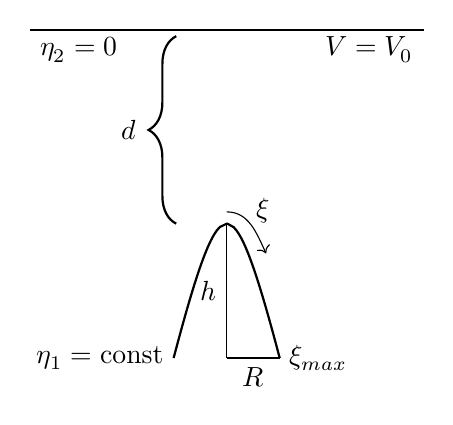
\begin{tikzpicture}
  \def\ximax{2.0}
  \def\etatip{-0.975}
  \def\afoci{1.75}
  
  \pgfmathsetmacro{\Rbx}{\afoci * sqrt((\ximax)^2 - 1) * sqrt(1 - (\etatip)^2)}
  \pgfmathsetmacro{\Rby}{\afoci * \ximax * \etatip - 0.75}
  \coordinate (R_base) at ($(\Rbx, \Rby)$);
  
  \pgfmathparse{\afoci * \ximax * \etatip - 0.75}
  \coordinate (tipbot) at ($(0.0, \pgfmathresult)$);
  
  \pgfmathsetmacro{\tiptopy}{\afoci * 1.0 * \etatip - 0.75}
  \coordinate (tiptop) at ($(0.0, \tiptopy)$);
  
  \draw[thick] (-2.5, 0.0) node[below, right, yshift=-0.25cm] {\(\eta_2 = 0\)} -- (2.5, 0.0) node[below, left, yshift=-0.25cm] {\(V = V_0\)};
  \draw[thick, samples=40, join=round] plot[domain=\ximax:1] ({\afoci * sqrt((\x)^2 - 1) * sqrt(1 - (\etatip)^2)}, {\afoci * \x * \etatip - 0.75} )
                                         -- plot[domain=1:\ximax] ({-\afoci * sqrt((\x)^2 - 1) * sqrt(1 - (\etatip)^2)}, {\afoci * \x * \etatip - 0.75} ) node[left] {\(\eta_1 = \mathrm{const}\)};
  
  \draw[thick, decorate, decoration={brace,amplitude=10pt}, xshift=-4pt, yshift=0pt] (-0.5, \tiptopy) -- (-0.5, -0.075) node [black, midway, xshift=-0.6cm] {\(d\)};
  
  \pgfmathsetmacro{\tipside}{\afoci * 1.25 * \etatip - 0.75}
  \coordinate (xiarr1) at ($(0.0, \tiptopy+0.15)$);
  \coordinate (xiarr2) at ($(0.5, \tipside+0.05)$);
  \draw[->] (xiarr1) to[out=0, in=115] (xiarr2);
  \draw[white, opacity=0.0] (xiarr1) -- (xiarr2) node[black, opacity=1.0, midway, above, xshift=0.20cm, yshift=0.0] {\(\xi\)};
  
  
  \draw[] (tipbot) -- (R_base) node[midway, below] {\(R\)} node[right] {\(\xi_{max}\)};
  \draw[] (tipbot) -- (tiptop) node[midway, left] {\(h\)};
\end{tikzpicture}
    \caption{Coordinates}
    \label{fig:coords_Rh}
  \end{figure}
  We then have
  \begin{equation}\label{eq:tip-radius}
    R = a \sqrt{\xi_{max}^2-1}\sqrt{1-\eta_1^2}
  \end{equation}
  \begin{equation}\label{eq:tip-height}
    h = -a\xi_{max}\eta - d = -\left( d + a\xi_{max}\eta_1 \right)
  \end{equation}
  and also
  \begin{equation}\label{eq:tip-eta}
    \eta_1 = -\frac{d}{a}
  \end{equation}

  By inserting Equation~\eqref{eq:tip-eta} into Equation~\eqref{eq:tip-height} we get
  \begin{equation}\label{eq:tip-ximax}
    \xi_{max} = \frac{h}{d} + 1
  \end{equation}
  We can then use Equation~\eqref{eq:tip-ximax} and Equation~\eqref{eq:tip-radius} to obtain
  \begin{equation}\label{eq:tip-a}
    a = \sqrt{\frac{d^2R^2}{h^2 + 2dh} + d^2}
  \end{equation}

  It is possible to use Equations~\eqref{eq:tip-eta},~\eqref{eq:tip-ximax} and \eqref{eq:tip-eta} to keep
  the shape of the tip constant for all \(d\).
%
\subsection{Radius of Curvature}
  Radius of Curvature is
  \begin{equation}
    R = \left| \frac{\left( \left(\frac{\ud x}{\ud \xi}\right)^2 + \left(\frac{\ud z}{\ud \xi}\right)^2 \right)^{\frac{3}{2}}}{\frac{\ud x}{\ud \xi} \frac{\ud^2 z}{\ud \xi^2} - \frac{\ud z}{\ud \xi} \frac{\ud^2 x}{\ud \xi^2}} \right| \, .
  \end{equation}
  Set \(\phi = 0\) and \(\eta = \eta_1\), we then have
  \begin{equation}
    \frac{\ud^2 x}{\ud \xi^2} = - a \frac{\sqrt{1-\eta_1^2}}{(\xi^2-1)^{\frac{3}{2}}}
  \end{equation}
  and
  \begin{equation}
    \frac{\ud^2 z}{\ud \xi^2} = 0\, .
  \end{equation}
  Therefore,
  \begin{equation}
    R = \left| \frac{a}{\eta_1} \frac{(\xi^2 - \eta_1^2)^{\frac{3}{2}}}{\sqrt{1-\eta_1^2}} \right| \, .
  \end{equation}
  If \(\xi = 1\) and \(\eta_1 = -\frac{a}{d}\) then
  \begin{equation}
    R = \frac{a^2}{d} - d\, .
  \end{equation}
%
\subsection{Normal Vector to surface}
  Starting with
  \begin{equation}
    \xi = \frac{1}{2a}\left( \sqrt{x^2 + y^2 + (z+a)^2} + \sqrt{x^2 + y^2 + (z-a)^2} \right)
  \end{equation}
  and inserting this into
  \begin{equation}
    z = a\xi\eta = \frac{\eta}{2} \left( \sqrt{x^2 + y^2 + (z+a)^2} + \sqrt{x^2 + y^2 + (z-a)^2} \right)\, .
  \end{equation}
  Now solve for \(z\) to obtain
  \begin{equation}
   z = f(x,y) = \frac{\pm\eta}{\sqrt{1-\eta^2}} \sqrt{x^2 + y^2 + a(1-\eta^2)}\, .
  \end{equation}
  The normal vector the point \((x_0, y_0)\) is then
  \begin{equation}
    \vec{N} = [f_x(x_0, y_0),\, f_y(x_0, y_0),\, -1]\, ,
  \end{equation}
  or
  \begin{equation}
   \vec{N} = \left[\frac{\eta}{\sqrt{1-\eta^2}} \frac{x_0}{\sqrt{x_0^2 + y_0^2 + a^2(1-\eta^2)}},\, \frac{\eta}{\sqrt{1-\eta^2}} \frac{y_0}{\sqrt{x_0^2 + y_0^2 + a^2(1-\eta^2)}},\, -1\right]\, .
  \end{equation}
  This vector points into the surface. Its norm is
  \begin{equation}
   |\vec{N}|^2 = \frac{1}{1-\eta^2} - \frac{a^2\eta}{x_0^2 + y_0^2 + a^2(1-\eta^2)}\, .
  \end{equation}
%
% %\clearpage
% \cleardoublepage
% %
% \subsection{Simpson's rule in 2D}
%   \begin{equation}
%    I = \int_{1}^{\xi_0} \int_{0}^{2\pi} h_{\xi} h_{\phi}\, j(\xi, \phi)\, \ud \phi\, \ud \xi\, .
%   \end{equation}
%   \begin{equation}
%    I = A a^2 \sqrt{1 - \eta^2} \int_1^{\xi_0} \int_{0}^{2\pi} \sqrt{\xi^2 - \eta^2} F^2(\xi, \phi) e^{-B/F(\xi,\phi)}\, \ud \phi\, \ud \xi\, .
%   \end{equation}
%   Set \(D = Aa^2\sqrt{1-\eta^2}\), \(f(\xi,\phi) = \sqrt{\xi^2 - \eta^2}F^2(\xi, \phi) e^{-B/F(\xi, \phi)}\), \(h = \frac{\xi_0 - 1}{2n}\) and \({k = \frac{2\pi}{2m}}\).
%   Simpson's rule is then
%   \begin{equation}\begin{split}
%     I &= \frac{D}{9}hk \Big\{ f(1,0) + f(1,2\pi) + f(\xi_0, 0) + f(\xi_0, 2\pi)\\
%                       &+ 4 \sum_{i=1}^n f(\xi_{2i-1}, 0) + 2\sum_{i=1}^{n-1} f(\xi_{2i}, 0) + 4\sum_{i=1}^n f(\xi_{2i-1}, 2\pi) + 2\sum_{i=1}^{n-1} f(\xi_{2i}, 2\pi)\\
%                       &+ 4\sum_{j=1}^m f(1, \phi_{2j-1}) + 2\sum_{j=1}^{m-1}f(1, \phi_{2j}) + 4\sum_{j=1}^m f(\xi_0, \phi_{2j-1}) + 2\sum_{j=1}^{m-1} f(\xi_0, \phi_{2j})\\
%                       &+ 16 \sum_{i=1}^n\sum_{j=1}^m f(\xi_{2i-1}, \phi_{2j-1}) + 8\sum_{i=1}^{n-1}\sum_{j=1}^m f(\xi_{2i}, \phi_{2j-1})\\
%                       &+ 8\sum_{i=1}^n\sum_{j=1}^{m-1} f(\xi_{2i-1}, \phi_{2j}) + 4\sum_{i=1}^{n-1}\sum_{j=1}^{m-1} f(\xi_{2i}, \phi_{2j}) \Big\}\, .
%   \end{split}\end{equation}
%
\cleardoublepage
\subsection{Circuit elements}
\begin{figure}[!ht]
  \centering
  \begin{circuitikz} \draw
    (0, -2) to[twoport, v^<=\(V_d\), *-*](0, 2) to[R, l_=\(R\), i<_=\(I\), v^=\(V_R\), *-*] ((2, 2) to[battery1, v=\(V_0\), *-*] (2, 0) to[C, l_=\(C\), v^=\(V_c\), *-*] (2, -2) -- (0, -2);
  \end{circuitikz}
  \caption{Circuit}
\end{figure}
For the circut we have
\begin{equation}
 V_d(t) = V + V_c(t)\, ,
\end{equation}
or
\begin{equation}
 V_c(t) = V_d(t) - V\, .
\end{equation}
For the capacitor
\begin{equation}
 I(t) = C\frac{d V_c(t)}{d t} = C \frac{d V_d(t)}{dt}\, ,
\end{equation}
because \(V\) is constant. Integration from \(0\) to \(t\) then gives
\begin{equation}
  V_d(t) = V_d(0) + C\int_0^t I(t^\prime) dt^\prime\, ,
\end{equation}

\cleardoublepage
\section{Cylindrical Geometry}

\subsection{Electric Field}
The Laplace equation in cylindrical coordinates is
\begin{equation}
 \nabla^2\Phi = \frac{1}{r}\frac{\delta}{\delta r}\left( r \frac{\delta\Phi}{\delta r}\right)
              + \frac{1}{r^2}\frac{\delta^2\Phi}{\delta \theta^2} + \frac{\delta^2\Phi}{\delta z} = 0\, .
\end{equation}
Due to symmetry in \(\theta\) and \(z\) we have
\begin{equation}
 \Phi = \Phi(r)\, ,
\end{equation}
or
\begin{equation}
 \nabla^2\Phi(r) = \frac{1}{r}\frac{\delta}{\delta r}\left( r \frac{\delta\Phi(r)}{\delta r}\right) = 0\, .
\end{equation}
Integration yields,
\begin{equation}
  \frac{\delta \Phi(r)}{\delta r} = \frac{A}{r}\, ,
\end{equation}
where \(A\) is a constant. A second integration then gives,
\begin{equation}
  \Phi(r) = A\ln(r) + B\, ,
\end{equation}
where \(B\) is also a constant.
\begin{figure}[!h]
  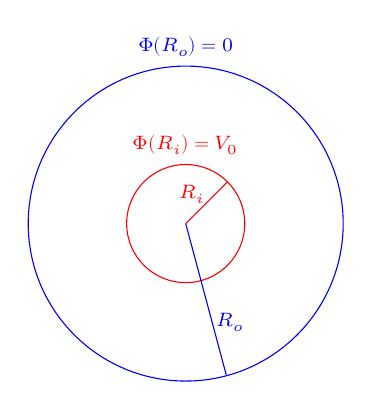
\begin{tikzpicture}
    \draw[red] (0, 0) circle (0.75cm);
    \draw[blue] (0, 0) circle (2.0cm);

    \draw[red] (0, 0) -- (45:0.75cm) node[midway, left, font=\scriptsize, xshift=3pt, yshift=3pt] {\(R_i\)};
    \draw[blue] (0, 0) -- (-75:0.75cm);
    \draw[blue] (-75:0.75cm) -- (-75:2.0cm) node[midway, right, font=\scriptsize, xshift=-2.5pt, yshift=2pt] {\(R_o\)};

    \node[font=\scriptsize, above, red] at (90:0.75cm) {\(\Phi(R_i) = V_0\)};
    \node[font=\scriptsize, above, blue] at (90:2.00cm) {\(\Phi(R_o) = 0\)};
  \end{tikzpicture}
  \centering
  \caption{A schematic illustration of the system.}
  \label{fig:system}
\end{figure}
The boundary conditions seen in Fig.~\ref{fig:system} are \(\Phi(R_i) = V_0\) and \(\Phi(R_o) = 0\). Using them to solve for the constants gives
\begin{equation}
  B = V_0\frac{\ln(R_o)}{\ln(R_o/R_i)}\, ,
\end{equation}
and
\begin{equation}
  A = \frac{V_0}{\ln(R_i/R_o)}\, .
\end{equation}
The electric field is then
\begin{equation}
 \vec{E} = - \vec{\nabla}\Phi
 = -\left(\frac{\delta \Phi}{\delta r}\hat{r} + \frac{1}{r}\frac{\delta\Phi}{\delta \theta}\hat{\theta} + \frac{\delta\Phi}{\delta z}\hat{z} \right)\, ,
\end{equation}
or
\begin{equation}
 \vec{E} = \frac{V_0}{\ln(R_o/R_i)}\frac{\hat{r}}{r}
         = \frac{V_0}{\ln(R_o/R_i)} \frac{\cos(\theta)\hat{x} + \sin(\theta)\hat{y}}{r}\, .
\end{equation}

\subsection{Emission}
The emission process checks the angle between the positon vector (black solid line) and the acceleration (\textcolor{violet}{violet} dashed line) (see Fig.~\ref{fig:angle}). If the angle \(\theta\) is greater than \(\pi/2\) then emission can occur.
\begin{figure}[!h]
  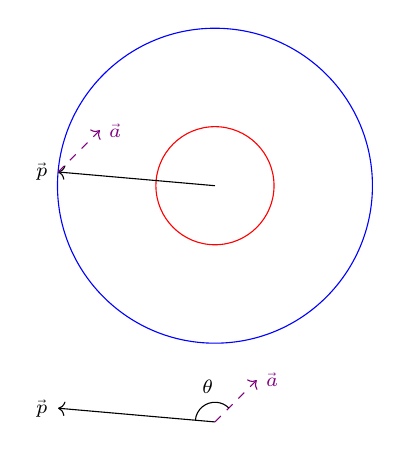
\begin{tikzpicture}
    \draw[red] (0, 0) circle (0.75cm);
    \draw[blue] (0, 0) circle (2.0cm);

    \draw[black, ->] (0:0) -- (175:2.0cm) node[left, font=\scriptsize] {\(\vec{p}\)};
    \draw[violet, dashed, ->] (175:2.0cm) -- ++(45:0.75cm) node[right, font=\scriptsize] {\(\vec{a}\)};

    \begin{scope}[yshift=-3cm]
     \draw[black, ->] (0:0) -- (175:2.0cm) node[left, font=\scriptsize] {\(\vec{p}\)};
     \draw[violet, dashed, ->] (0:0cm) -- ++(45:0.75cm) node[right, font=\scriptsize] {\(\vec{a}\)};
     \draw (175:0.25cm) arc (175:45:0.25cm) node[above, midway, font=\scriptsize] {\(\theta\)};
    \end{scope}
  \end{tikzpicture}
  \centering
  \caption{Angle between position and acceleration.}
  \label{fig:angle}
\end{figure}

\cleardoublepage\printbibliography
\end{document}
